\selectlanguage{italian}%

\section{Soluzione}


\subsection{Schematici}

Il sommattore essenzialmente � costituito da un numero di carry select
cell, di dimensione identiche (� possibile scegliere la dimensione
della cella) che calcolano le somma parziali e propagano i riporti
alle celle successive, il numero di celle da istanziare � data dalla
dimensione della cella e dal numero di bit su cui viene effettuata
la somma, una cella � costituita da due Ripple Carry Adder uno avente
carry in ingresso pari ad uno ed un altro pari a zero, di seguito
si determinano valori caratteristici del sommatore considerando una
carry select cell di dimensione pari a quattro bit.\begin{figure}[H]
	\centering
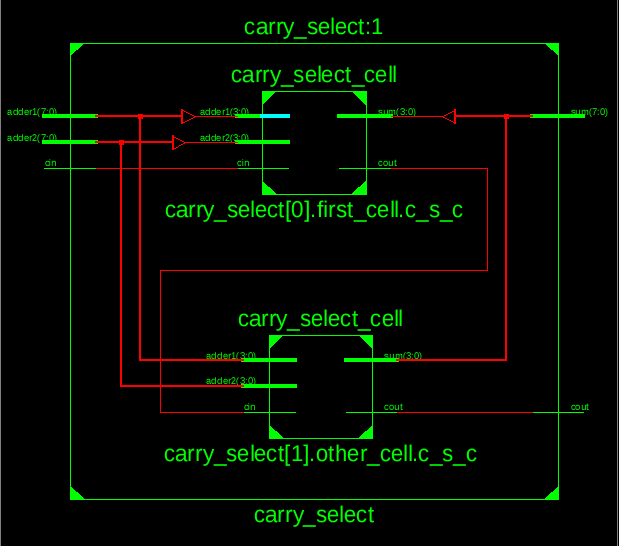
\includegraphics[scale=0.6]{esercizio11/images/carry_select.png}
	\caption{Carry Select Adder}
\end{figure}
\begin{table}[H]
\noindent\begin{minipage}[t]{1\columnwidth}%
\begin{tabular}{|c|c|c|c|}
\hline 
Numero di bit operandi & Numero di slice & Numero di four LUT & Tempo di calcolo\tabularnewline
\hline 
\hline 
4 & 5 & 10 & 6,853 ps\tabularnewline
\hline 
8 & 12 & 21 & 7,467 ps\tabularnewline
\hline 
16 & 24 & 43 & 8,521 ps\tabularnewline
\hline 
32 & 48 & 87 & 9,984 ps\tabularnewline
\hline 
\end{tabular}%
\end{minipage}
\end{table}

Confrontando i risultati con il sommatore Ripple Carry Adder, \ref{Dati ripple carry}
il numero di slice occupate � pressoch� lo stesso tranne nel primo
caso, invece il numero delle LUT � maggiore, dovute alle interconnessioni
che permettono ai Ripple Carry Adder di avere carry in ingresso pari
ad uno o zero e a quelle per collegare i vari carry in uscita. I tempi
di calolo sono migliori in tutti i casi tranne che nell 'ultimo che
sono pressoch� gli stessi, l' uguaglianza del tempo di calcolo nell'
ultimo caso con quello del Ripple Carry Adder � dovuto che il carry
select avendo una cella di dimensione quattro all' aumentare del numero
di operandi, aumentano il numero di celle istanziate, il tempo di
attesa dell' ultima cella diventa sempre maggiore e tende ad essere
comparabile con quello di un Ripple Carry Adder.

\subsection{Codice}

\href{run:progetti/carry_select_adder/carry_select_adder.xise}{Carry Select Adder ISE}

\selectlanguage{italian}%

